%%%%%%%%%%%%%%%%%%%%%%%%%%%%%%%%%%%%%%%%%%-PREAMBLE-%%%%%%%%%%%%%%%%%%%%%%%%%%%%%%%%%%%%%%%%%%

% Packages

\documentclass{assignment}
\usepackage[pdftex]{graphicx} % FIGURES
\usepackage{xcolor}
\definecolor{LightGray}{gray}{0.95}
\usepackage{fancyvrb, minted} % CODE
\usepackage[letterpaper, margin = 2.5cm]{geometry} % PAGE SIZE AND MARGINS
\usepackage[T1]{fontenc} % Important for automatic accents and special writing symbols
\usepackage{amsmath, amsfonts, amssymb} % Equations, special characters, and symbols
\usepackage{hyperref, url}  % Links and hyperlinks in the document
\usepackage{fancyhdr}
\usepackage{csvsimple}
\usepackage{listings}
\usepackage{color}
\usepackage{booktabs}
\usepackage{float} % for H placement specifier
\usepackage{dsfont}

\usepackage{multirow}


\definecolor{dkgreen}{rgb}{0,0.6,0}
\definecolor{gray}{rgb}{0.5,0.5,0.5}
\definecolor{mauve}{rgb}{0.58,0,0.82}

\lstset{frame=tb,
  language=Python,
  aboveskip=3mm,
  belowskip=3mm,
  showstringspaces=false,
  columns=flexible,
  basicstyle={\small\ttfamily},
  numbers=none,
  numberstyle=\tiny\color{gray},
  keywordstyle=\color{blue},
  commentstyle=\color{gray},
  stringstyle=\color{dkgreen},
  breaklines=true,
  breakatwhitespace=true,
  tabsize=3
}

\usepackage{dsfont}

%-----------------------------------------LABELS--------------------------------------------

\student{CID: 02528663}                             % NAME
\semester{Summer Term}                                % SEMESTER (202X A/B)
\date{\today}                                   % Date (Modify to DD/MM/YYYY)

\courselabel{MATH70076 Data Science}          % COURSE CODE AND NAME
\exercisesheet{}{}     % EXERCISE SHEET NUMBER AND TITLE

\school{Data Science}          % MAJOR (Physics, the best major)
\university{Assignment 2}         % THE MIGHTY UNIVERSITY

%%%%%%%%%%%%%%%%%%%%%%%%%%%%%%%%%%%%%%%%%%-DOCUMENT-%%%%%%%%%%%%%%%%%%%%%%%%%%%%%%%%%%%%%%%%%%%%

\begin{document}

\section{Genre Classification: Introduction}

In this report, my main focus will be to find the "best" classification model to predict genre of a song given features of the song (danceability, energy, loudness, acousticness, instrumentalness, liveness, valence and tempo). I will consider three classes of models: K Nearest Neighbors Classifier (KNN), Decision Tree Classifier and Multilayer Perceptron (MLP). I will individually train "best" model of each class and compare them in "Results" part of this report.

\section{Data pre-processing}

Original dataset contains over 150 different genres. To make the problem simpler, I grouped them into following categories:
\begin{itemize}
    \item \textbf{Electronic Dance Music}: edm, house, electro, trance, techno, dubstep, drum-and-bass, deep-house, detroit-techno, minimal-techno, progressive-house and breakbeat.

    \item \textbf{Rock}: alt-rock, rock, indie, indie-pop, punk, punk-rock, hard-rock, metal, heavy-metal, black-metal, death-metal and grunge.

    \item \textbf{Hip-Hop and R\&B}: hip-hop, r-n-b, trap.

    \item \textbf{Pop}: pop, electro-pop, synth-pop, k-pop, pop-film and power-pop.

    \item \textbf{Latin \& Reggae/Dancehall}: latin, reggaeton, salsa, samba, reggae and dancehall

    \item \textbf{Funk and Disco}: funk, disco and groove.

    \item \textbf{Other}: all other genres that are not listed above.
\end{itemize}

After this grouping, \textbf{Other} is the almost 5 times bigger than next category (\textbf{Rock} with over 11k songs), therefore to make the dataset more balance I keep only 20k of \textbf{Other} (selected through random sampling). The final counts are shown in Figure \ref{fig:music_categories_counts}.

\medskip

The distribution of the predicting features are given in Figure \ref{fig:histograms_of_features}. We can observe that all categories are distributed in range [0,1] apart from loudness and tempo. Moreover, some features are more uniformly distributed (valance), while loudness, speechiness, acousticness, instrumentalness and liveness are more "skewed" and take values in smaller "window" of values. I will standardise all the features to have mean 0 and standard deviation 1 to ensure that each feature contributes the same to prediction. 

\medskip

I am splitting the data into test dataset and train dataset (used for both training and validation) in 15/85 proportions. Note that I only use the train data to find scalar values and then use them on test data to avoid "data leakage".

\begin{figure}[H]
\centering
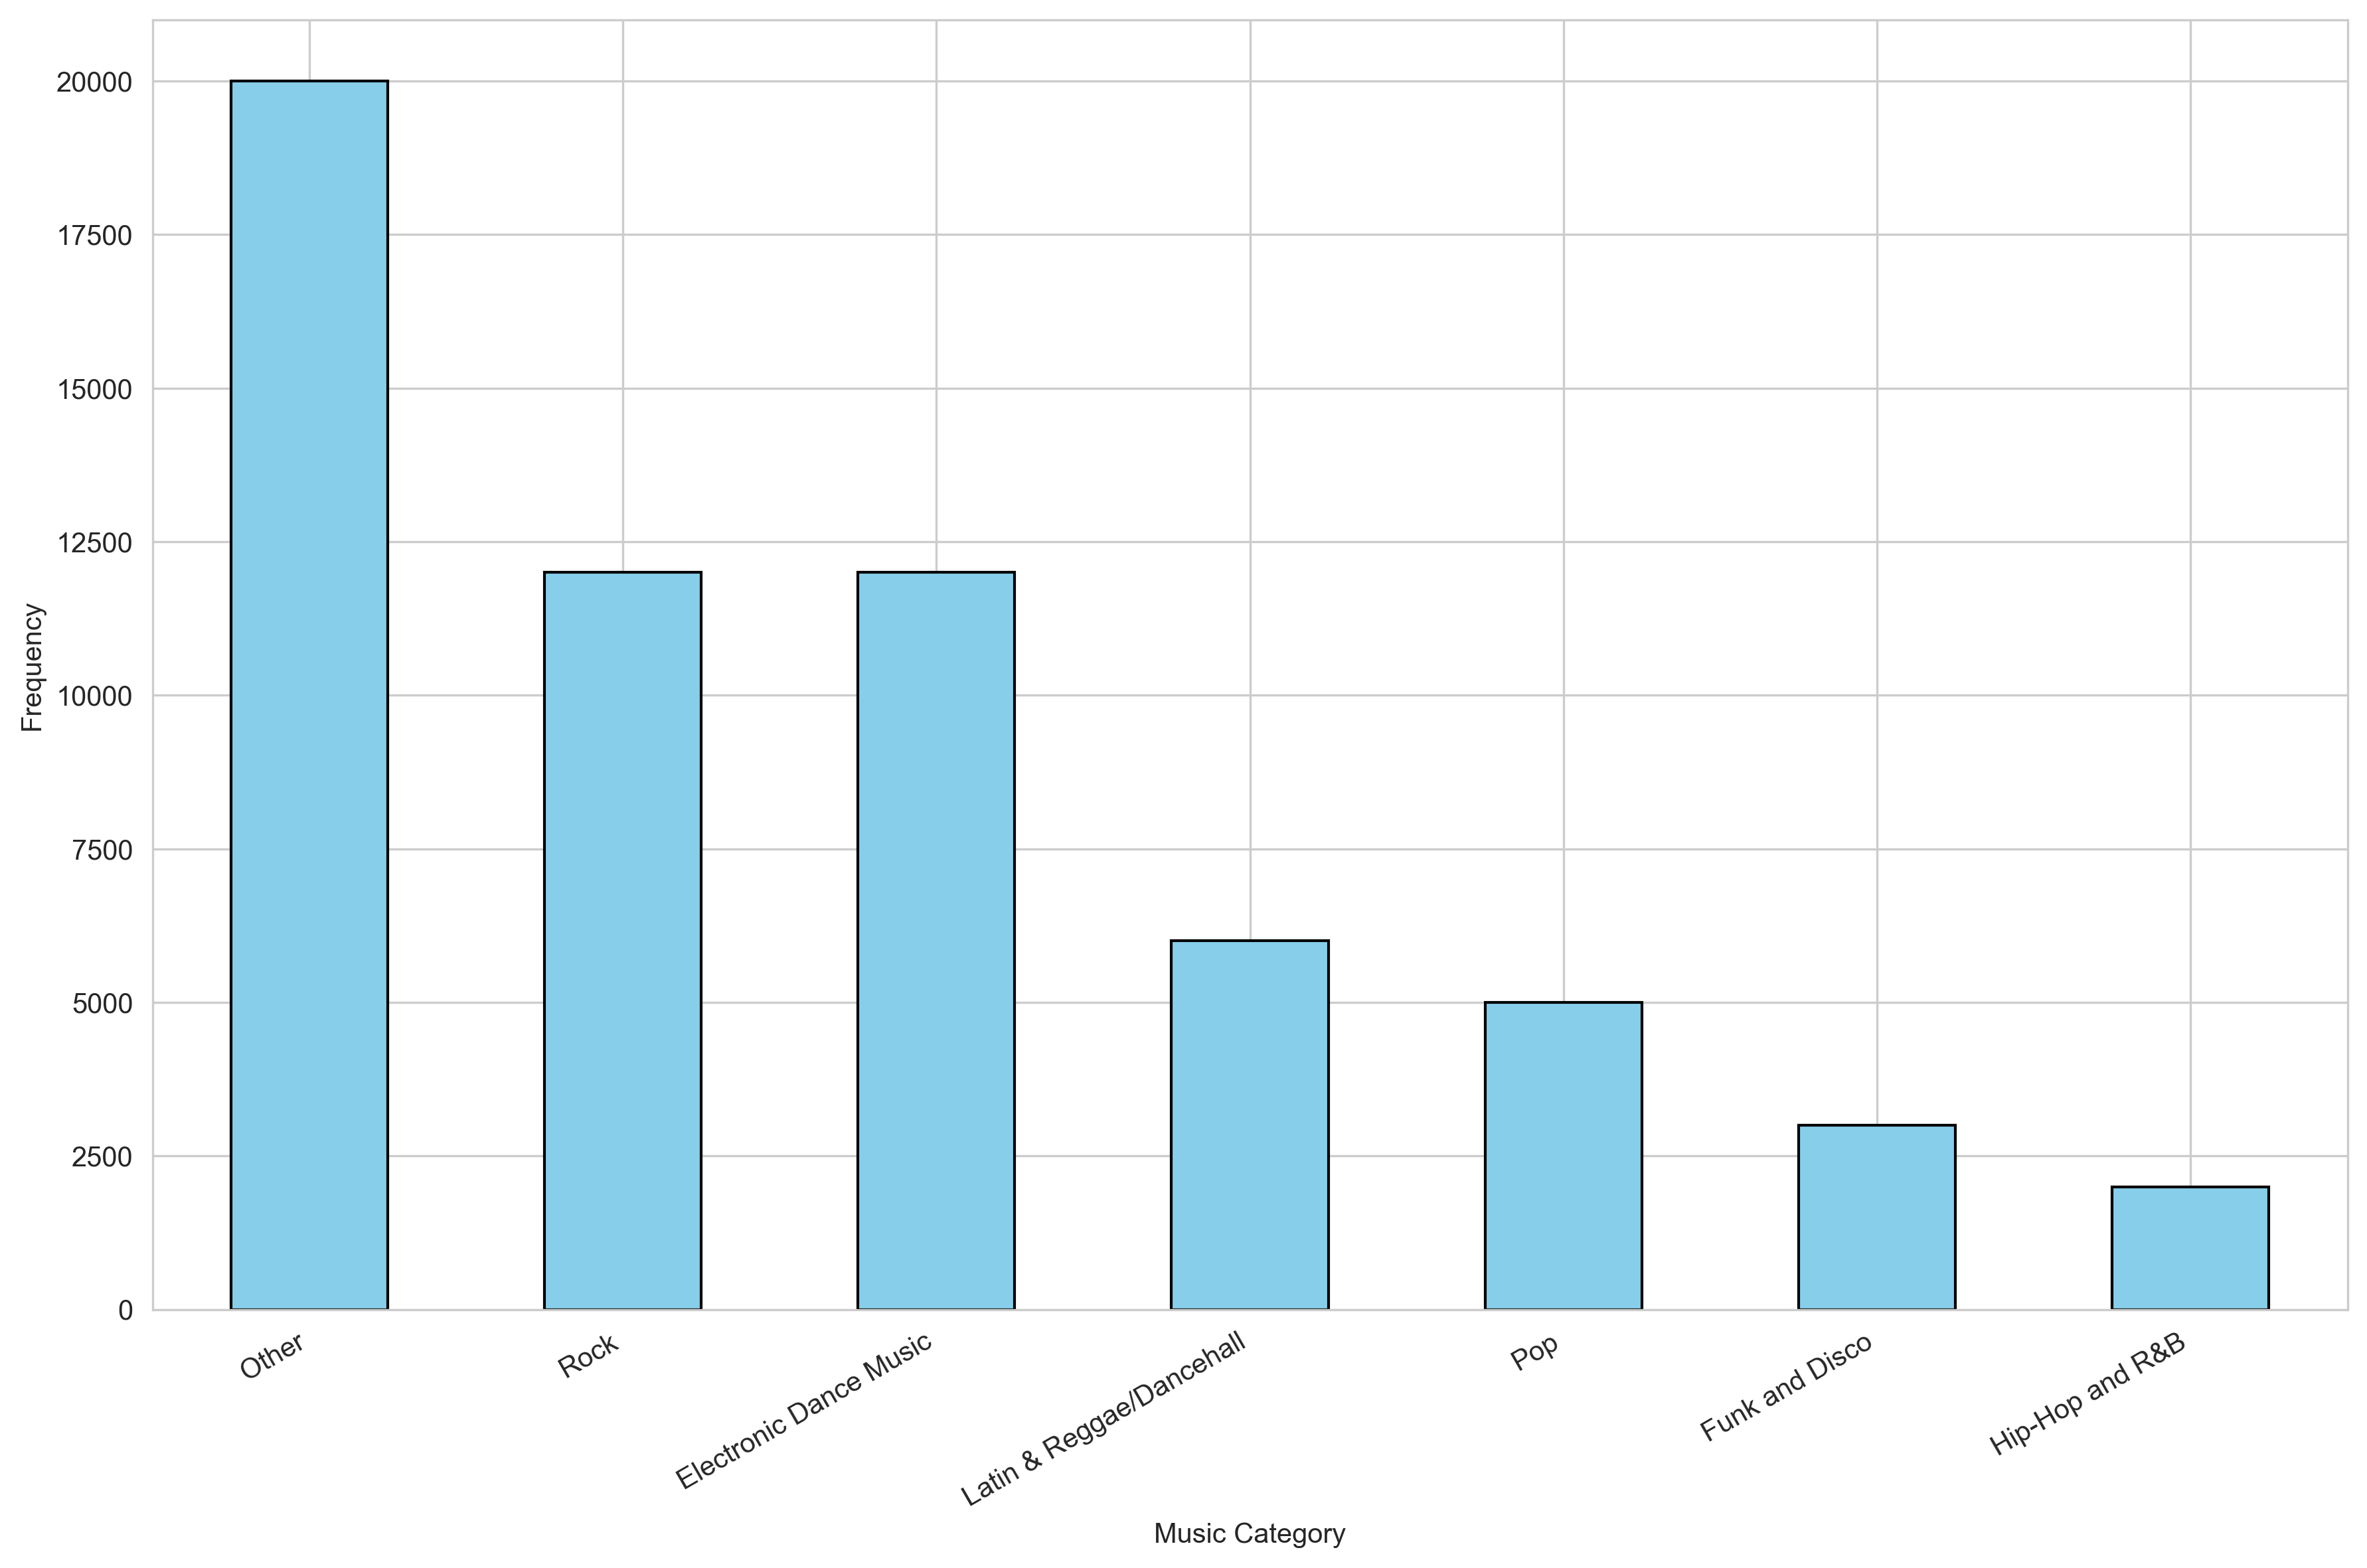
\includegraphics[width=0.9\linewidth]{music_categories_counts.png}
\caption{\label{fig:music_categories_counts}Counts of each music category after sub-sampling \textbf{Other} category.}
\end{figure}


\begin{figure}[H]
\centering
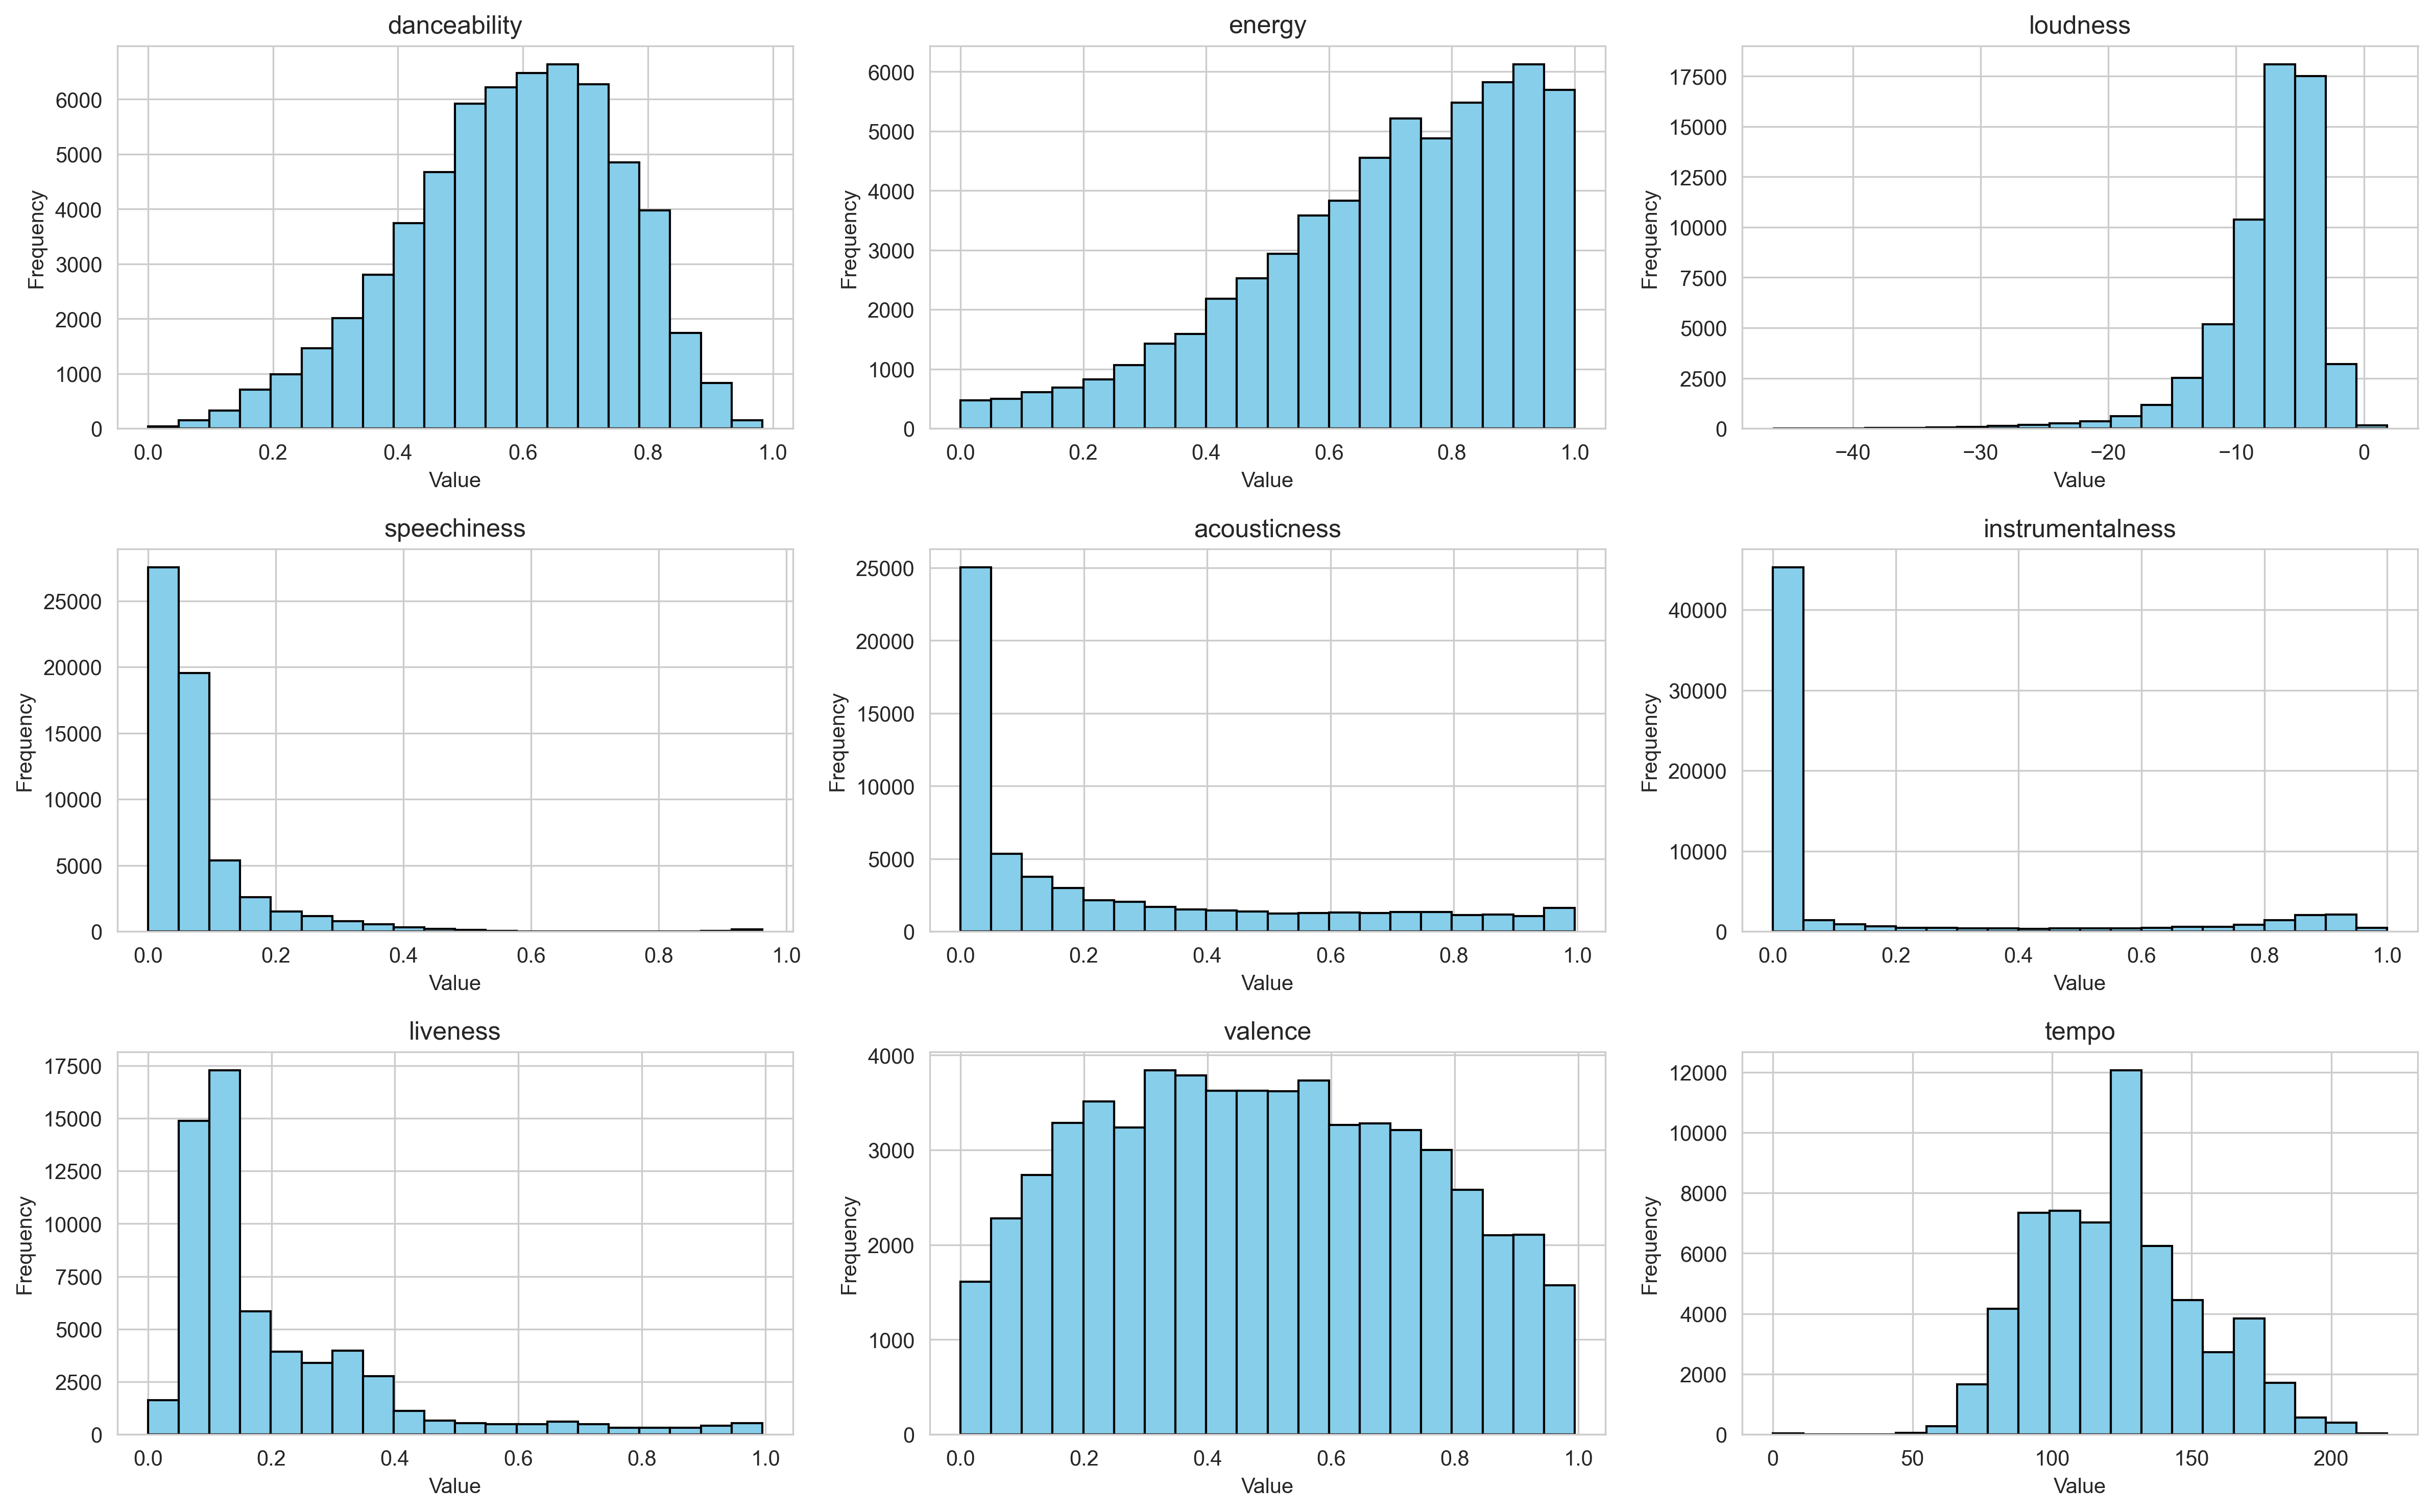
\includegraphics[width=0.9\linewidth]{histograms_of_features.png}
\caption{\label{fig:histograms_of_features}Histograms of each feature before standardisation.}
\end{figure}


\newpage

\section{Hyper-parameter experimentation}

\noindent\rule{16.5cm}{0.55pt}
\smallskip

The first model I introduce is the \textbf{K Nearest Neighbors (KNN) Classifier}, a non-parametric method used for classifying data points based on their similarity in feature space. KNN does not require explicit training but instead makes predictions based on the majority class among the K nearest neighbors of a query point.

I will experiment with two types of KNN classifiers:

\begin{enumerate}
    \item \textbf{Majority Vote-based KNN:} The predicted class $\hat{y}$ for a query point is determined by the majority class among its K nearest neighbors.

    \item \textbf{Distance-weighted KNN Classifier:} The predicted class $\hat{y}$ is calculated by weighting the contributions of each neighbor's class based on their distances to the query point. This is achieved using inverse distance weighting, where the weight $w_i$ for each neighbor is inversely proportional to its distance from the query point.
\end{enumerate}

For calculating the K nearest neighbors, I will experiment with using different distance metrics: Euclidean and Manhattan. In practice, our dataset is to big to "brute" force search through all the train data points to find the "closest" neighbors, thus I will use \texttt{KNeighborsClassifier} from \texttt{sklearn.neighbors} package to fit all the models as it uses \texttt{BallTree} which is designed for fast generalized of N-point problem.

\medskip

I will use 5-fold cross-validation accuracy to choose best hyper-parameters combination. Figure \ref{fig:KNN_classifier_hyperparameter_tuning_plot} shows cross-validation accuracy for odd K's in range 1 to 40 for four KNN classifiers combinations described above. We can observe that chose of K and distance had biggest impact on performance. The biggest cross-validation accuracy is achieved for Distance-weighted KNN Regression with Manhattan distance for K=33 (accuracy=0.5856). Furthermore, we can see the accuracy is extremely similar for any K above 13, thus we could potentially consider choosing smaller K if computational cost is our main concern. However, I will choose the model with the best accuracy performance.


\bigskip
\bigskip




\begin{figure}[H]
\centering
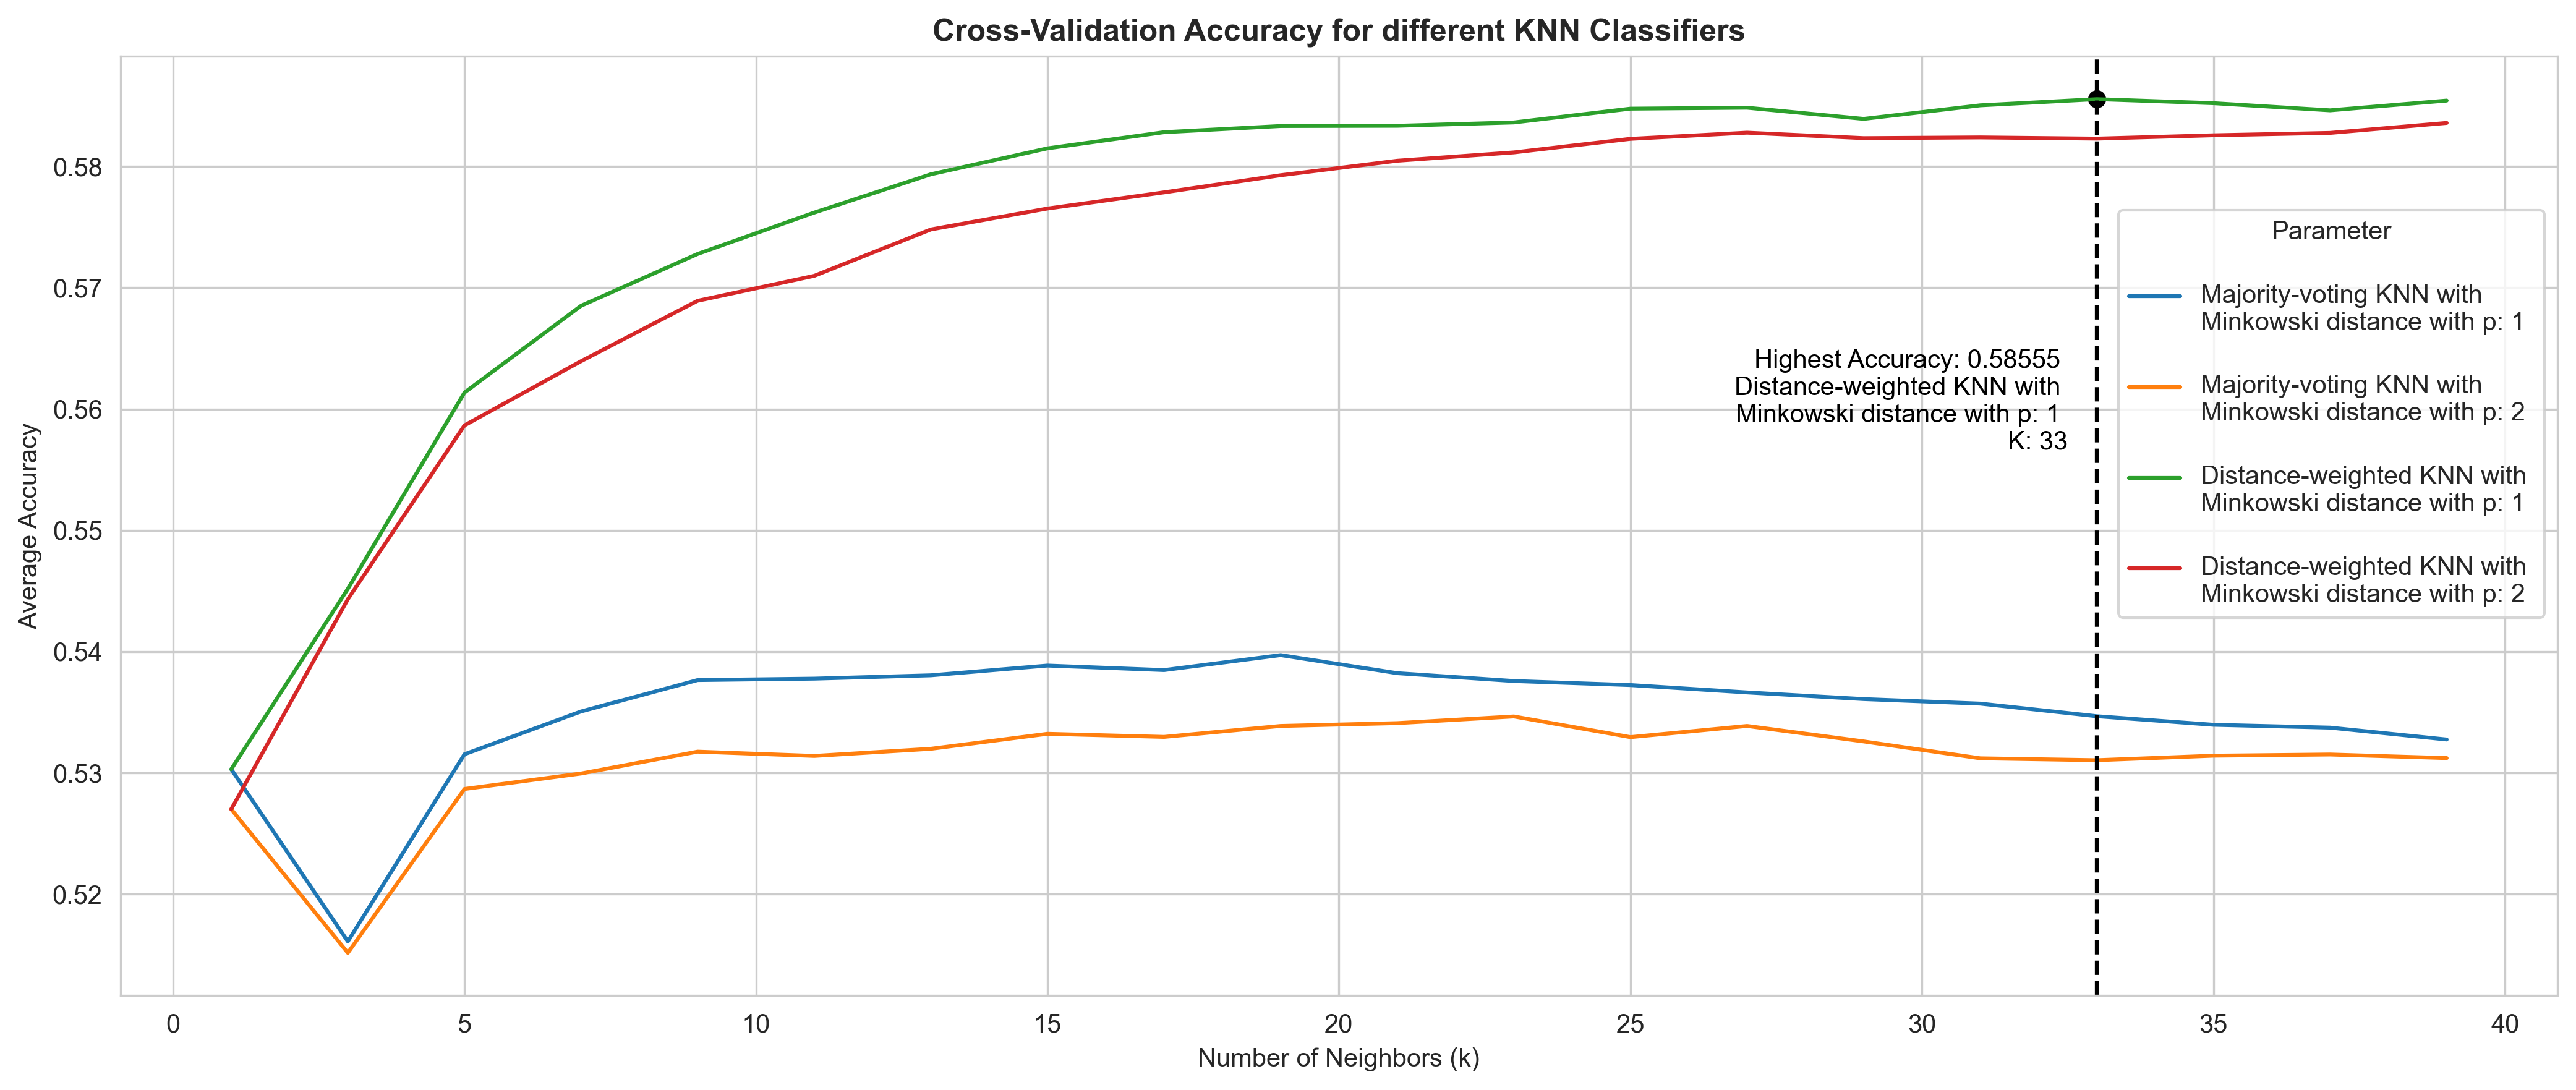
\includegraphics[width=0.9\linewidth]{KNN_classifier_hyperparameter_tuning_plot.png}
\caption{\label{fig:KNN_classifier_hyperparameter_tuning_plot}Cross-validation accuracy for different KNN methods against K. Note that Minkowski distance with p=1 corresponds to Manhattan distance and with p=2 to Euclidean distance. Maximal accuracy KNN is marked by black dashed line.}
\end{figure}


\newpage

\noindent\rule{16.5cm}{0.55pt}

\bigskip


The second model I introduce is the \textbf{Decision Tree Classifier}. It works by recursively partitions the feature space based on the values of input features, aiming to maximize Gini impurity at each split. Starting from the root node, the algorithm selects the best feature and threshold to split the dataset into subsets, iteratively creating branches that lead to leaf nodes representing class labels. 

\medskip

To classify new data points, the algorithm traverses the decision tree from the root node down to a leaf node, assigning the majority class label of the samples in that node as the predicted class.
\medskip

However, without a stopping criteria the trees get overly complex and are prone to over-fitting. Thus I we introduce complexity parameter $\alpha$ that regulates the trade-off between model simplicity and accuracy by selectively pruning the tree by removing branches that have little impact on the overall impurity reduction, thereby simplifying the tree structure. For hyper-parameter tuning, I grid-search 200 points of $\alpha$ in range $(10^{-6}, 10^{-1})$ equally spaced on logarithmic scale. I will use \texttt{sklearn.tree.DecisionTreeRegressor} to fit all the models.

\medskip


I will again use 5-fold cross-validation to compare the models. The results my experimentation are shown in Figure \ref{fig:Decision_Tree_classifier_hyperparameter_tuning_plot}. We can observe that the highest accuracy of 0.5352 was archived for $\alpha=9.12\times10^{-5}$. The final tree has depth of 20 with 671 decision leafs. As we increase the parameter $\alpha$ (making the tree grow "bigger"), the accuracy drastically falls to under 0.35 for $\alpha=0.1$. 
\bigskip
\bigskip





\begin{figure}[H]
\centering
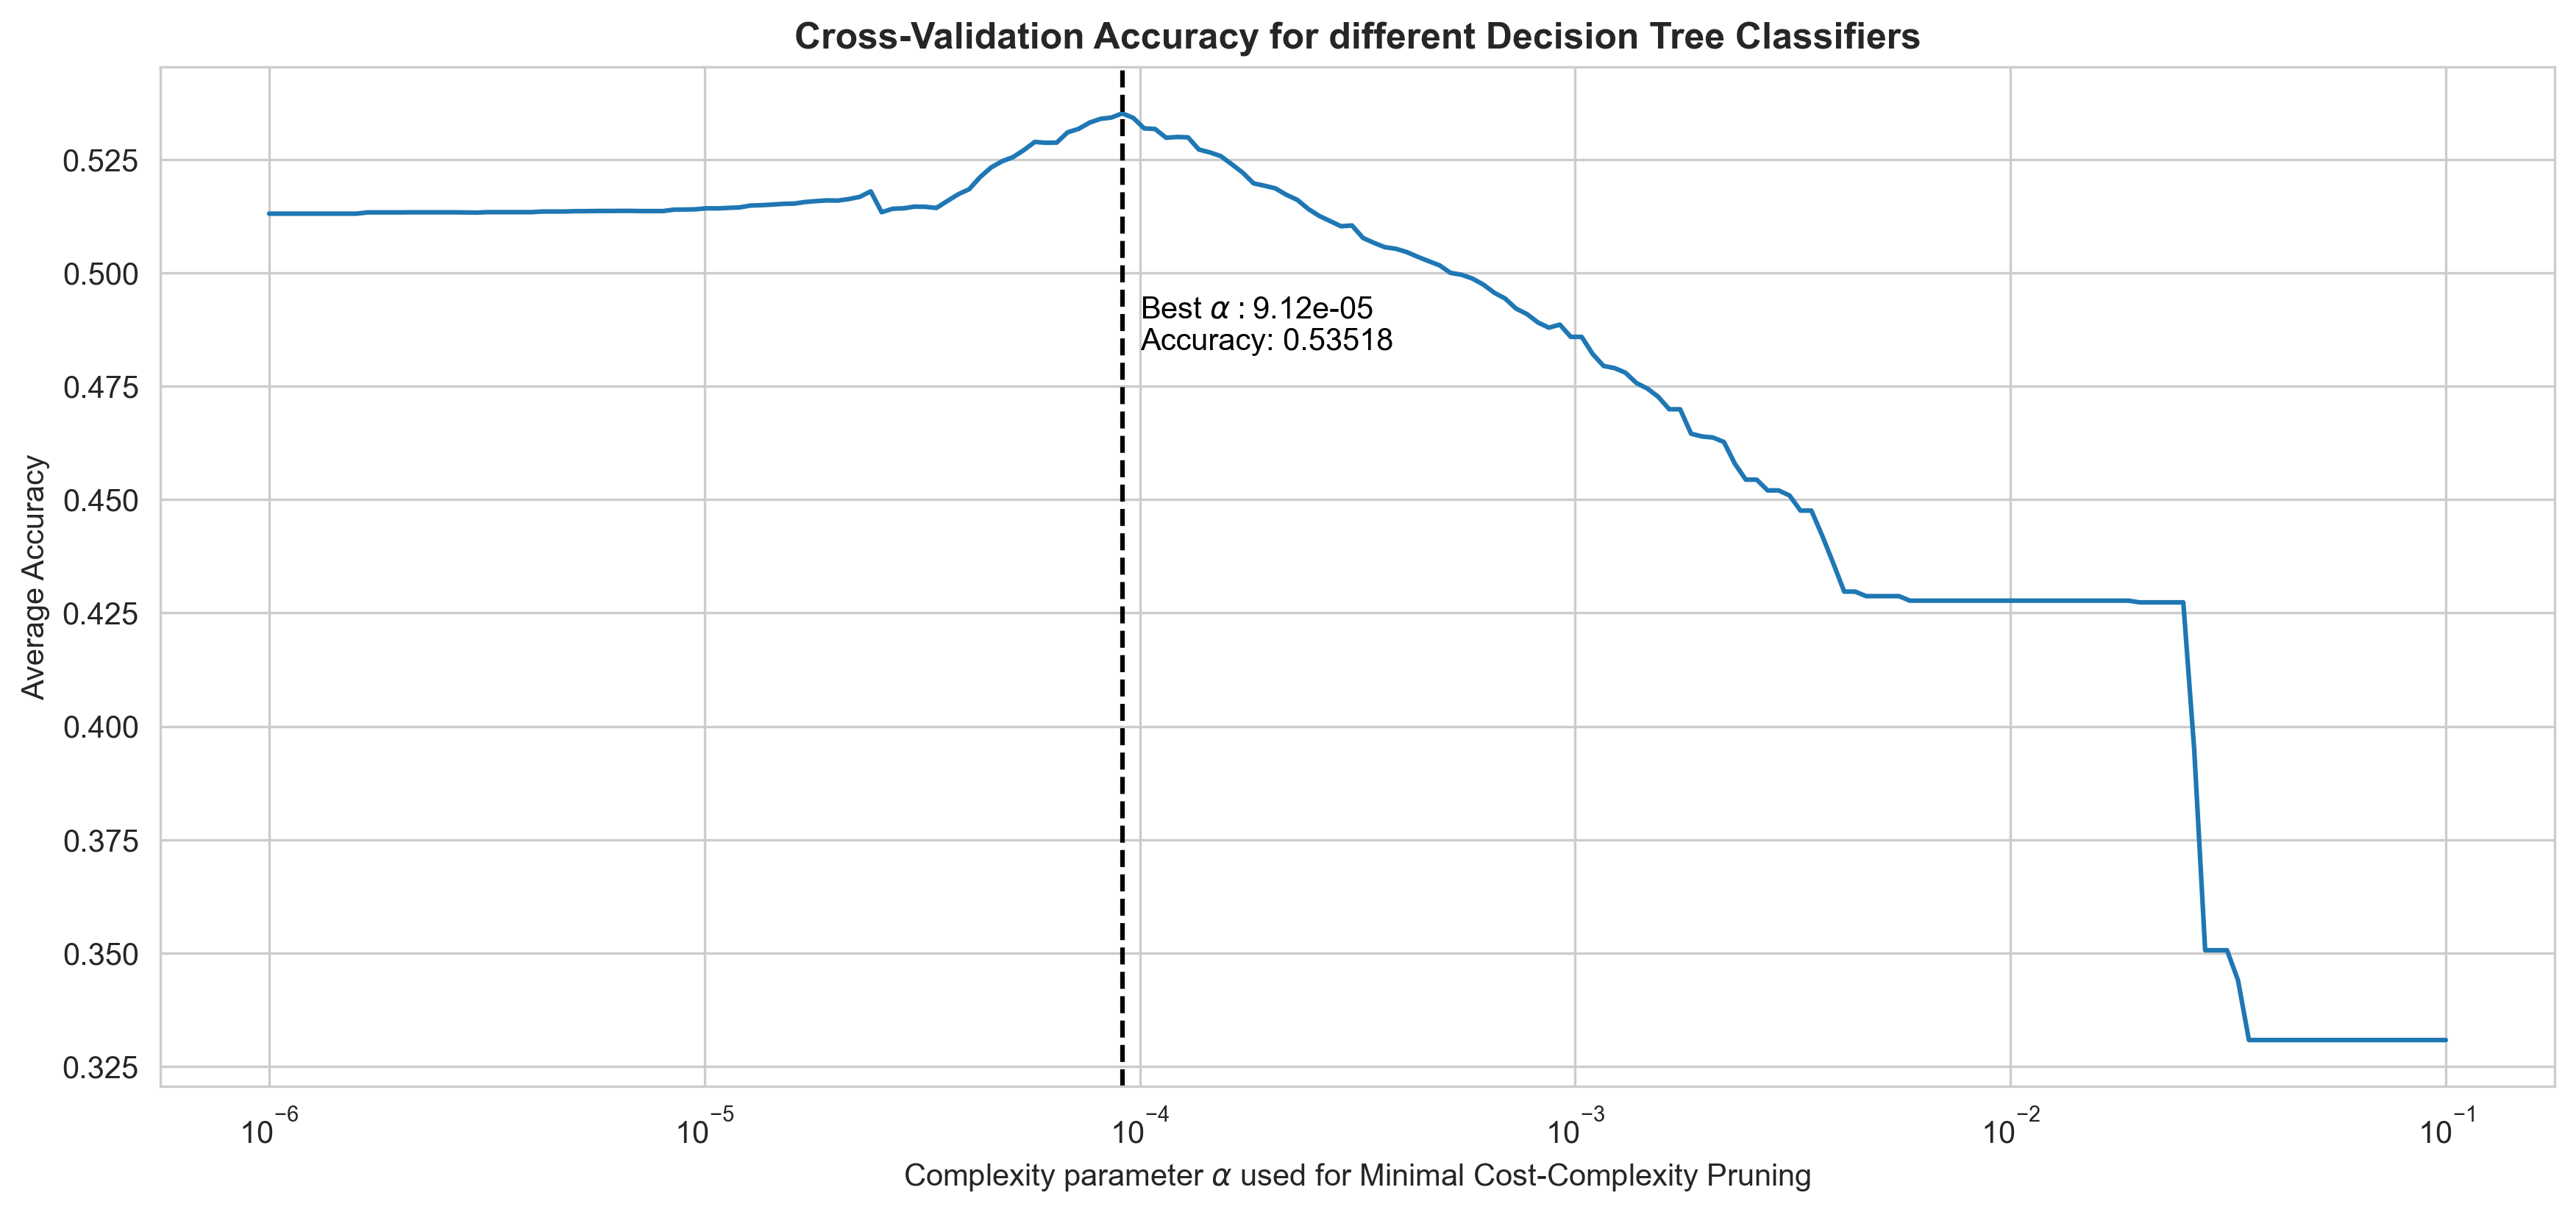
\includegraphics[width=0.9\linewidth]{Decision_Tree_classifier_hyperparameter_tuning_plot.png}
\caption{\label{fig:Decision_Tree_classifier_hyperparameter_tuning_plot}Plot of cross-validation accuracy as a function of hyper-parameter $\alpha$ which is used for selectively pruning. Black dashed line indicates $\alpha$ maximising the validation accuracy. Note that x-axis is on log skale.}
\end{figure}

\newpage

\noindent\rule{16.5cm}{0.55pt}
\smallskip

Third model I introduce is fully-connected \textbf{Multilayer Perceptron (MLP)}, which is a feedforward artificial neural network comprising multiple layers of interconnected neurons. I chose it model as MLP is a universal approximator, meaning it can approximate any function give it is "deep" and "wide" enough. The architecture consists of an input layer having  9 neurons (9 features), one or more hidden layers, and 7-neuron output layer (one for each class). Each neuron in the network is connected to every neuron in the adjacent layers.

\smallskip


The number of hidden layers and the number of neurons in each hidden layer hyper-parameters. Mathematically,

$$
z_j^{(l)} = \sum_{i=1}^{n^{(l-1)}} w_{ij}^{(l)} x_i^{(l-1)} + b_j^{(l)}
$$

$$
a_j^{(l)} = \sigma(z_j^{(l)})
$$

where $x_i^{(l-1)}$ represents the output of neuron $i$ in the previous layer, $w_{i j}^{(l)}$ is the weight connecting neuron $i$ to neuron $j$ in layer $l, b_j^{(l)}$ is the bias of neuron $j$ in layer $l, \sigma$ is the activation function, and $a_j^{(l)}$ is the output (activation) of neuron $j$ in layer $l$. I chose activation function for each hidden layer neuron to be RELU.


\smallskip

These models are trained through backpropagation using using gradient descent optimization to minimize a predefined loss function (categorical cross-entropy), iteratively adjusting the network's weights and biases. I will use Adam optimizer with learning rate being another hyper-parameter. I used \texttt{tensorflow} package to fit all the models.

\smallskip

Since training of MLP models is extremely dependent on initial starting conditions and the data used to train them (since the loss landscape of those models is extremely complex), I will use one predefined train/validation split (80/20) to train all of my MLP models. I will fit models with number of hidden layers in range 1 to 3 with number of neuron in each layer in $\{32,64,128\}$. For each model I will use four different learning rates \{0.1,0.01,0.001,0.0001\} with training batch size of 128 and show only the best model. Moreover, I employ early stopping with patience 20 on validation categorical cross-entropy (max 100 epochs), and select the model with smallest validation loss. 

\smallskip


The results are shown in Table (\ref{tab:MLP_val_loss}). We can observe that models performed extremely similar given their adequate learning rate. The smallest validation categorical cross-entropy is archived model consisting 1 hidden layer with 64 neurons each (1.389). This model was fitted using $10^{-4}$ learning rate archived its best validation loss at 50-th epoch (see Figure \ref{fig:best_model_training_plot}). It corresponds to 0.4843 validation accuracy. Moreover, We can observe that after 20 epoches the model make marginal improvements but it does not seem to overfits as validation loss stays close to training MSE throughout the training.

\bigskip

\begin{table}[H]
\centering
\begin{tabular}{|cc||rrr|}
\hline
 &  & \multicolumn{3}{c|}{\textbf{Number of Hidden Layers}} \\ \cline{3-5} 
 &  & \multicolumn{1}{c|}{1} & \multicolumn{1}{c|}{2} & \multicolumn{1}{c|}{3} \\ \hline \hline
\multicolumn{1}{|c|}{\multirow{3}{*}{{\textbf{\begin{tabular}[c]{@{}c@{}}Number of \\ Neutrons\end{tabular}}}}} & 32 & \multicolumn{1}{r|}{1.390} & \multicolumn{1}{r|}{1.393} & 1.394 \\ \cline{2-5} 
\multicolumn{1}{|c|}{} & 64 & \multicolumn{1}{r|}{\textbf{1.389}} & \multicolumn{1}{r|}{1.390} & 1.392 \\ \cline{2-5} 
\multicolumn{1}{|c|}{} & 128 & \multicolumn{1}{r|}{1.390} & \multicolumn{1}{r|}{1.391} & 1.393 \\ \hline
\end{tabular}
\caption{Table contains validation categorical cross entropy for MLP models with given number of hidden layer and number of neurons. Each value in the table represent the best validation categorical cross entropy the model scored throughout training across using four different learning rates of Adam optimizer \{0.01,0.001,0.0001,0.00001\} training for 100 epoches with patience 20. The best score is bold.}
\label{tab:MLP_val_loss}
\end{table}



\begin{figure}[H]
\centering
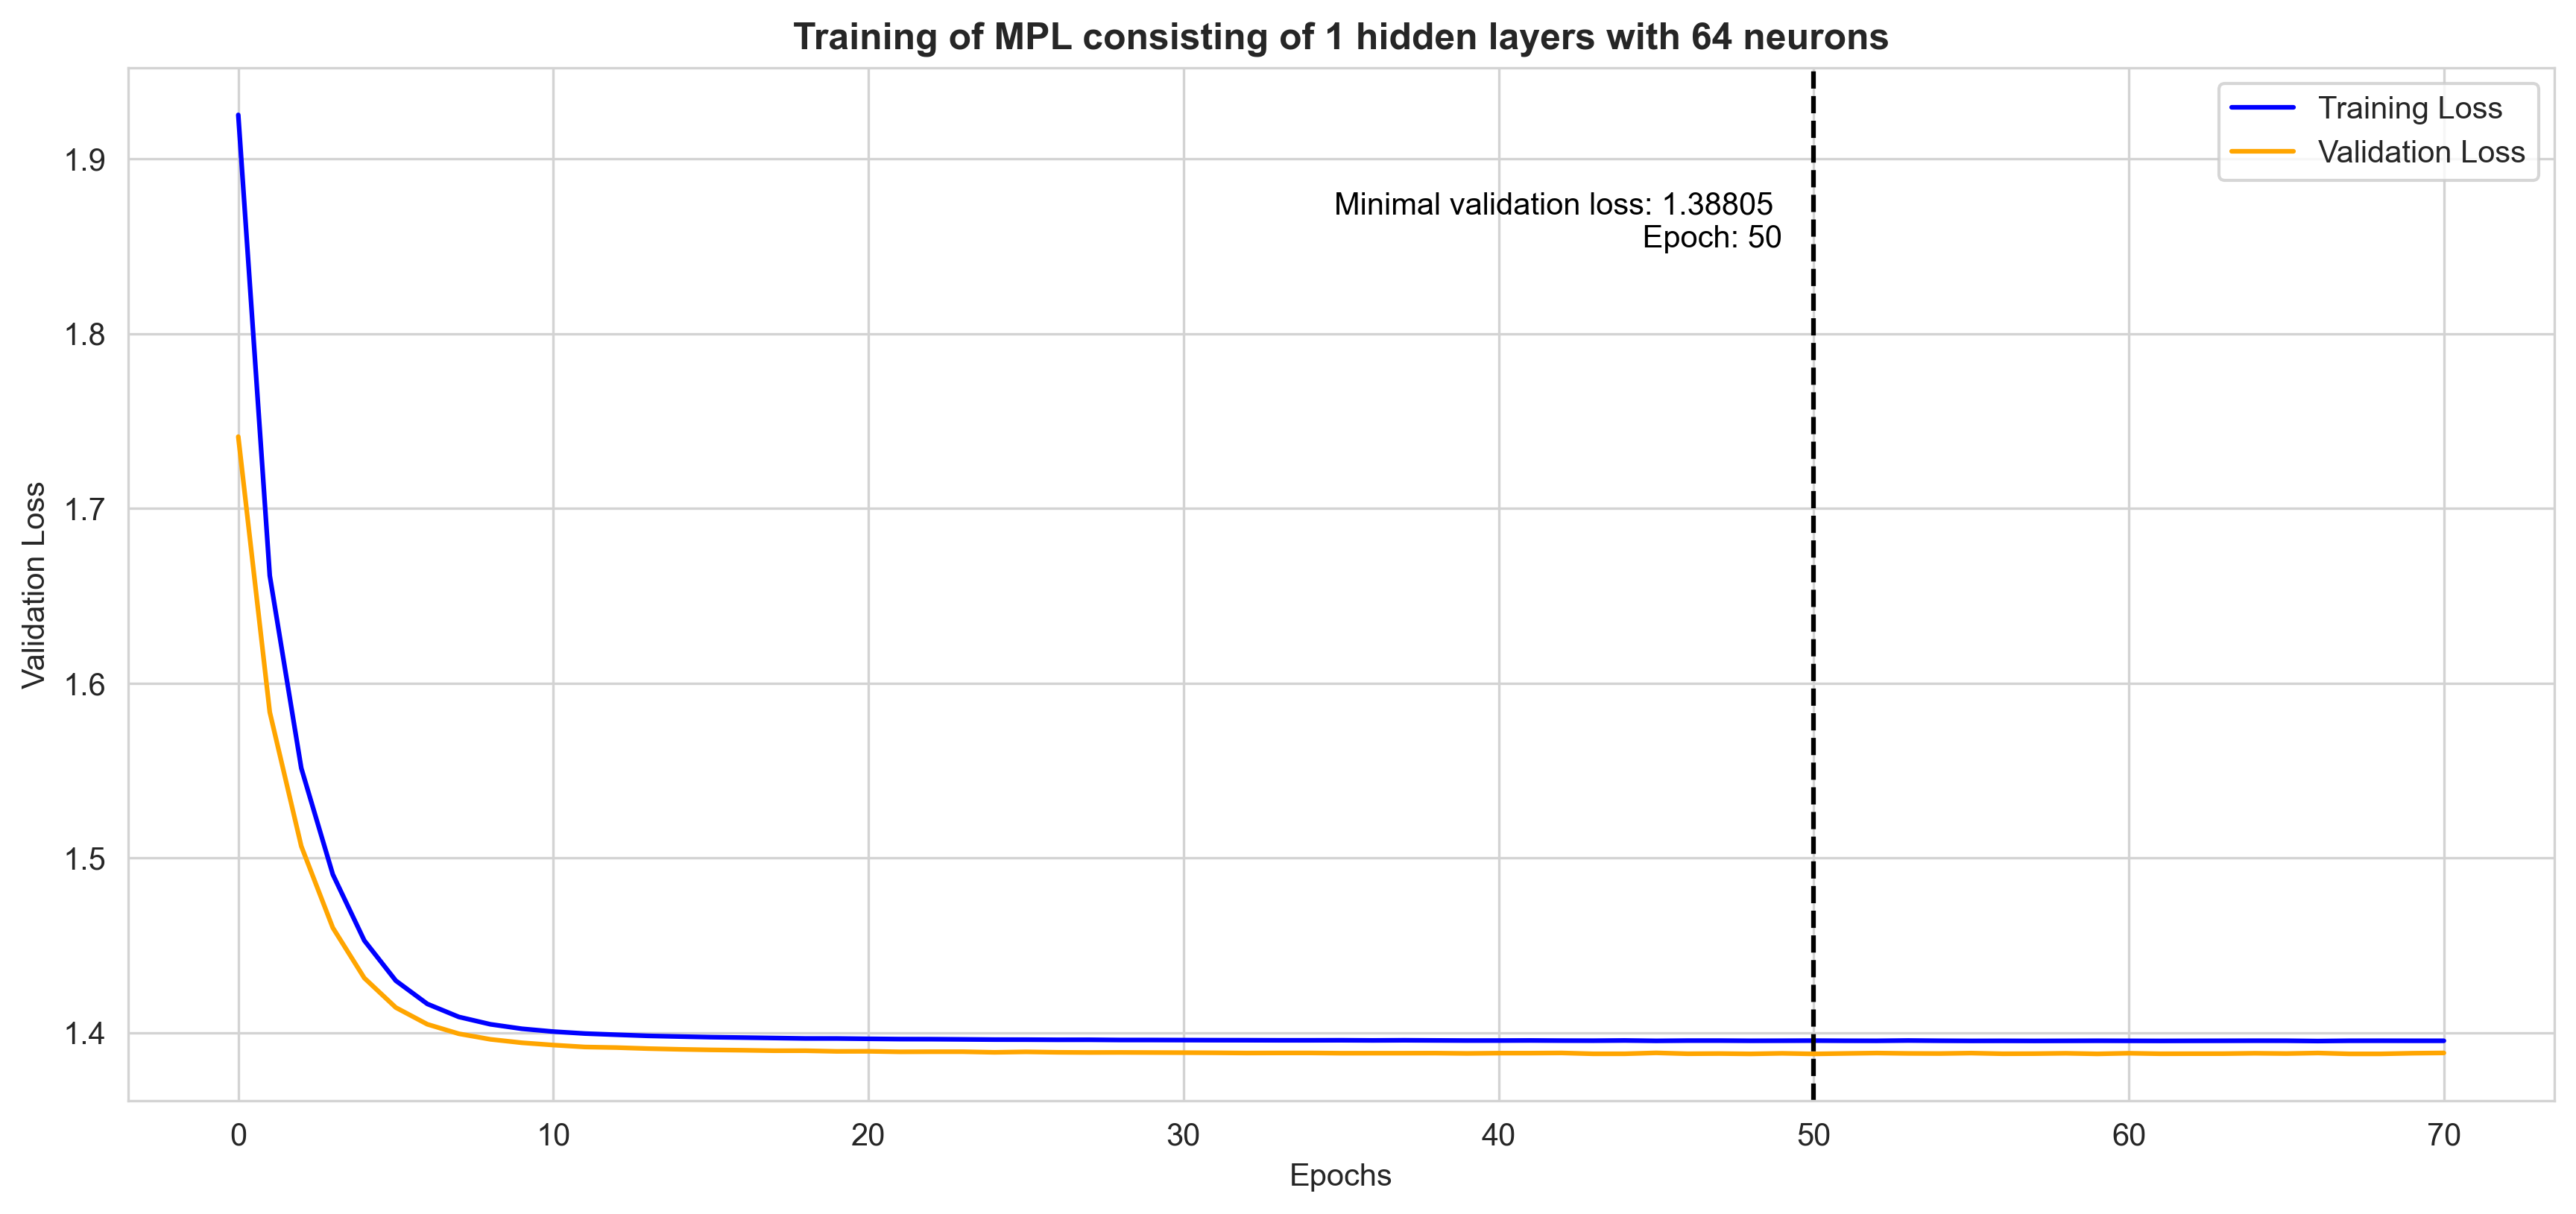
\includegraphics[width=0.9\linewidth]{best_model_training_plot.png}
\caption{\label{fig:best_model_training_plot}Plot shows training and validation loss (categorical cross-entropy) against epoch for MLP consisting of 1 hidden layer with 64 neurons. The learning rate in Adam optimizer was $10^{-4}$ for 100 epochs with patience of 20. Model finished after training after 70 epoches.}
\end{figure}

\section{Results}

The performance in terms of accuracy for selected models of each class is given in Table \ref{tab:all_test_acuraccy}. We can observe that the models test accuracy was better than the validation accuracy, proving that models were were not over-fitting the data. The highest test accuracy scored distance-weighted KNN classifier with K=33 and Manhattan distance function (0.5984). The worst performance across both test and validation is MLP classifier model.

\smallskip

We take a further look at Confusion Matrices in Figure \ref{fig:confusion_matrices}. We can observe that all models "avoided" predicting underrepresented genres as 'Funk and Disco', 'Hip-Hop and R\&B' and 'Pop'. 'Rock', 'Electronic Dance Music' and 'Other' were genres that were the most accurately predicted. Moreover, we can observe that most misclassification were classified as 'Other', which is the group with the most samples in our dataset. 

\smallskip

All in all, my recommendation is to use the distance-weighted KNN classifier with K=33 and Manhattan distance function as it showed the best performance in our hyper-parameter tuning and later testing. Notably, its interpretability stands out as a key advantage, allowing stakeholders to gain insights into the decision-making process. However, it does not come without its limitations. The most prominent disadvantages of KNN classifier is its high computational complexity and sensibility to noisy and irrelevant features. It is also important to point out that the model is far from perfect (0.5984 accuracy), making it a useful tool for prediction genres but its predictions should not be taken as absolute truth. 



\bigskip

\begin{table}[H]
\centering
\begin{tabular}{|l||r|r|r|}
\hline
 & \multicolumn{1}{c|}{\textbf{\begin{tabular}[c]{@{}c@{}}Decision Tree\\ Classifier\end{tabular}}} & \multicolumn{1}{c|}{\textbf{\begin{tabular}[c]{@{}c@{}}KNN\\ Classifier\end{tabular}}} & \multicolumn{1}{c|}{\textbf{\begin{tabular}[c]{@{}c@{}}MLP\\ Classifier\end{tabular}}} \\ \hline \hline
\multicolumn{1}{|c||}{\textbf{\begin{tabular}[c]{@{}l@{}}Test\\  Accuracy\end{tabular}}} & 0.5474 & 0.5984 & 0.4901 \\ \hline
\textbf{\begin{tabular}[c]{@{}l@{}}Validation\\  Accuracy\end{tabular}} & 0.5352 & 0.5856 & 0.4843* \\ \hline
\end{tabular}
\caption{Table contains test and validation accuracy for model selected during hyper-tuning. All values are rounded to 4 decimal points. *MLP validation accuracy calculated on one train/validation split (80/20), while all other validation accuracy's are calculated using 5-fold cross-validation.}
\label{tab:all_test_acuraccy}
\end{table}


\begin{figure}[H]
\centering
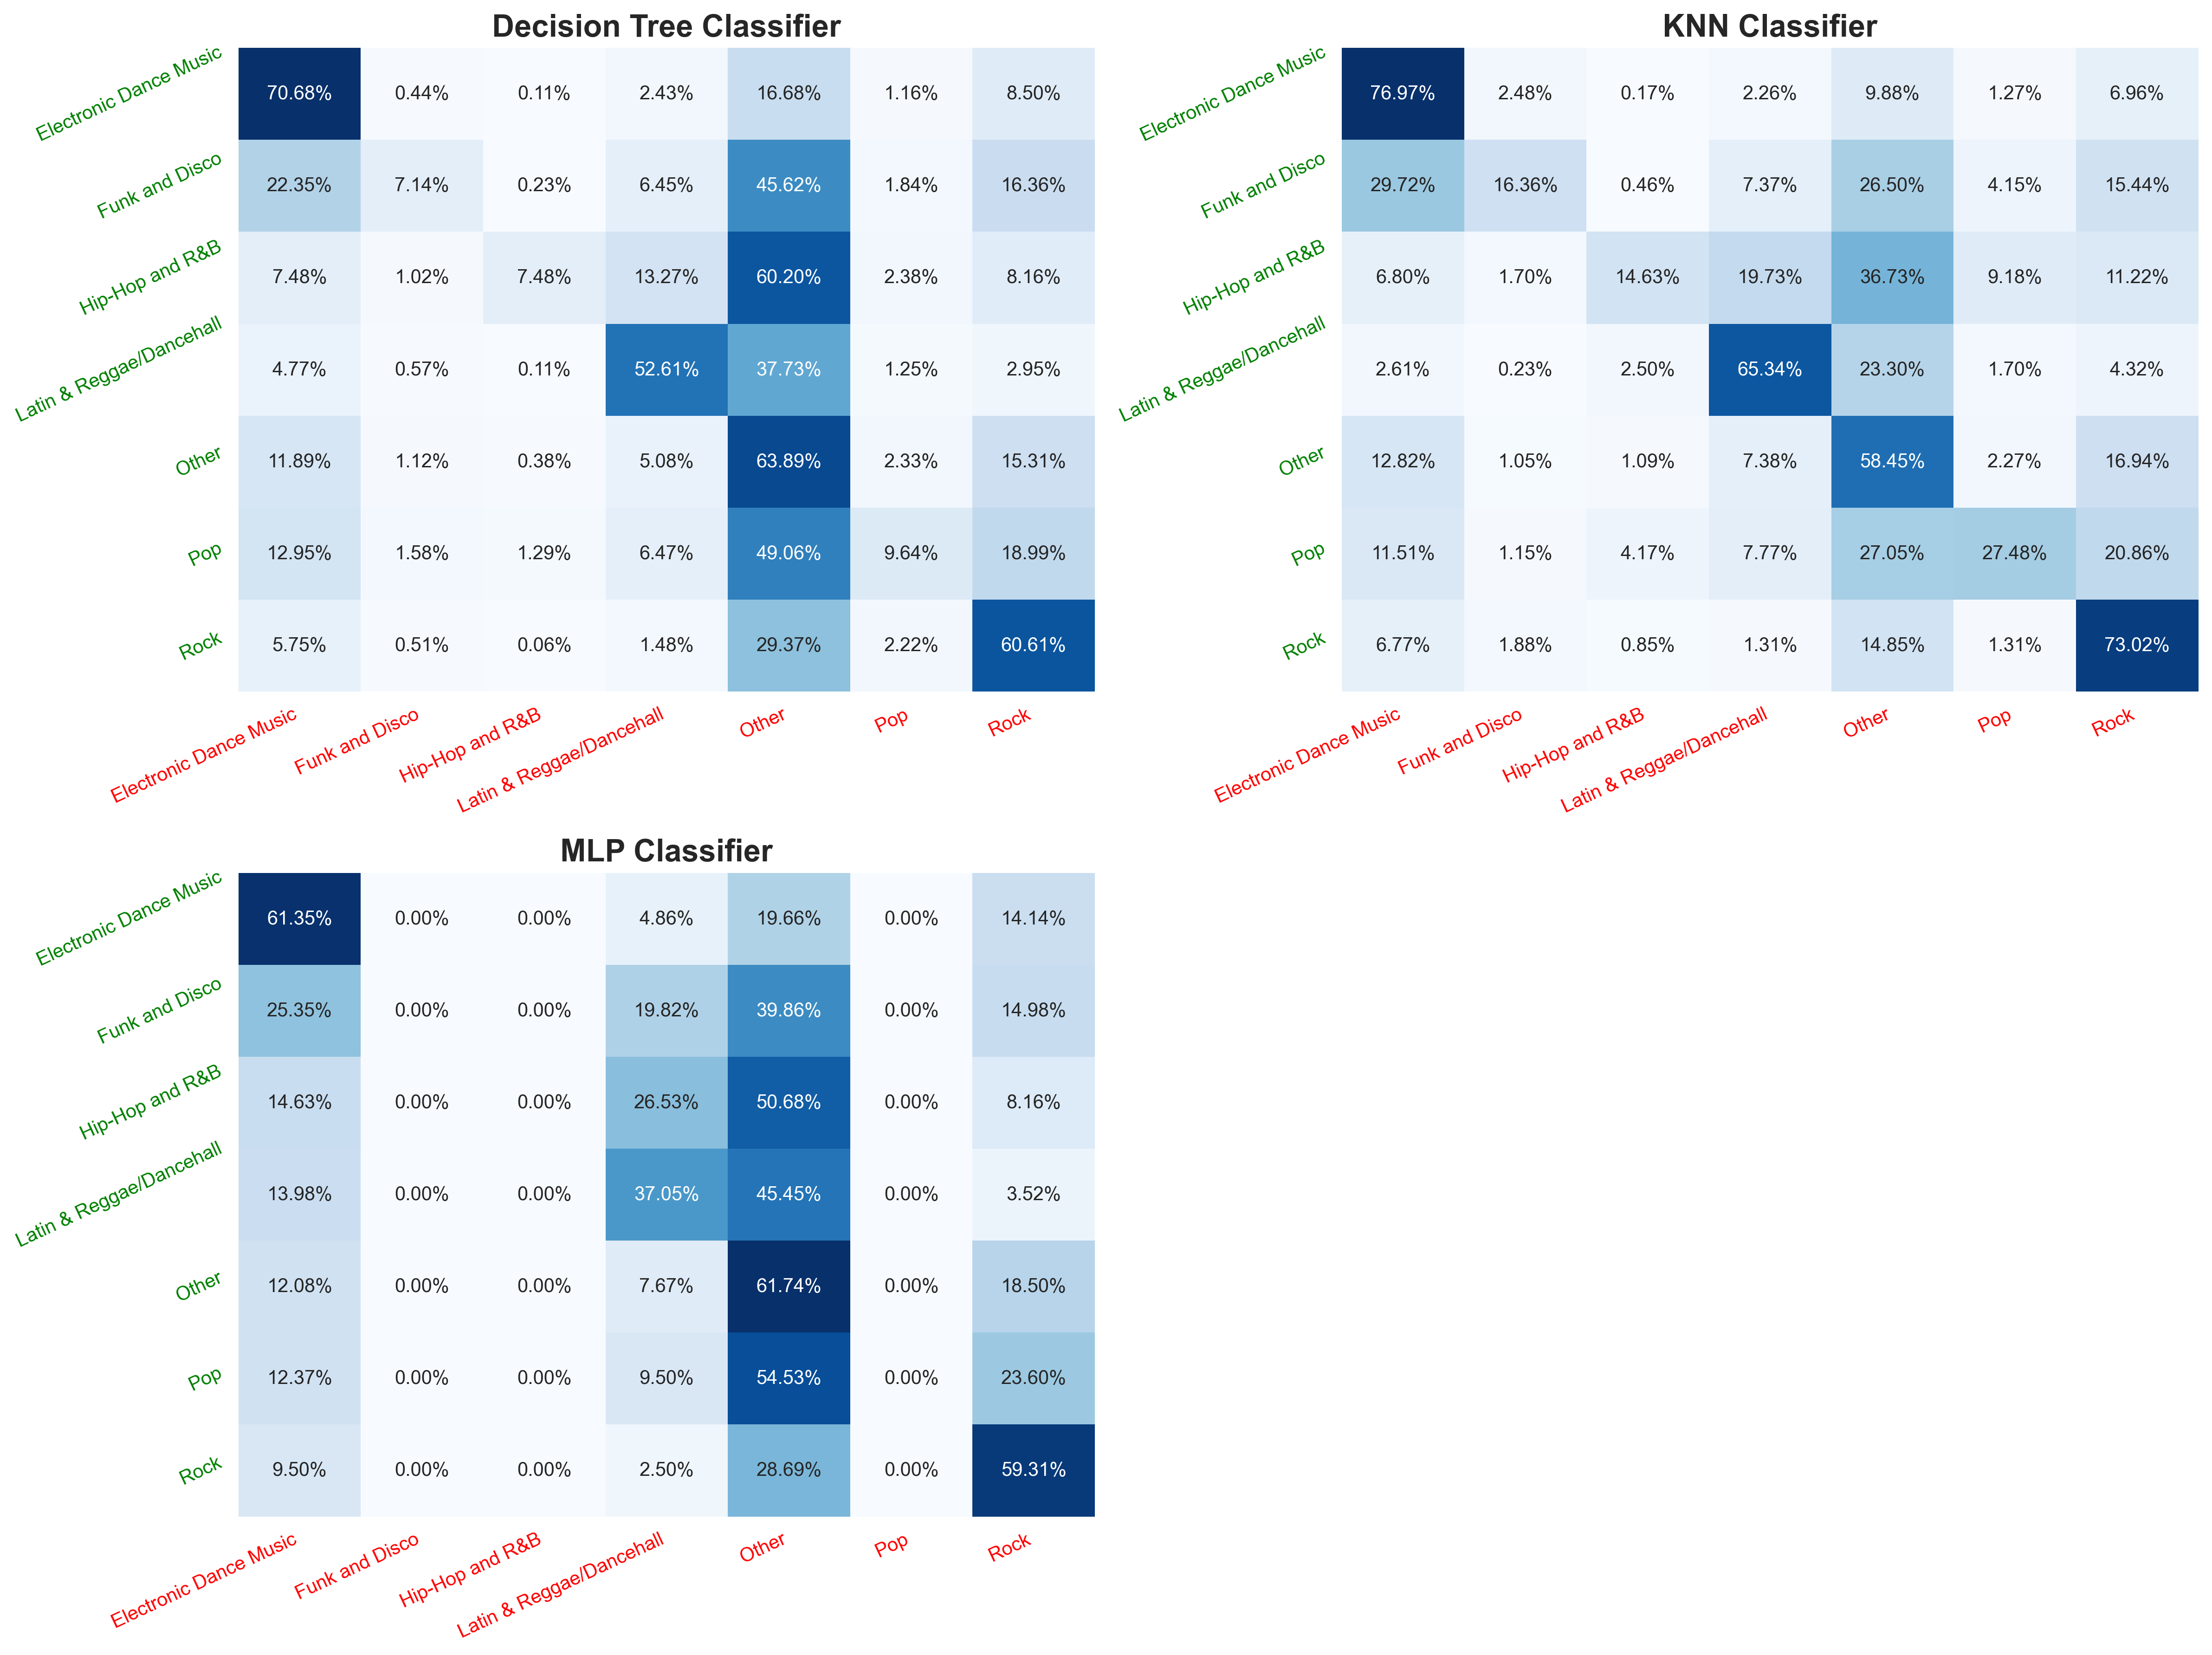
\includegraphics[width=0.9\linewidth]{confusion_matrices.png}
\caption{\label{fig:confusion_matrices}Confusion matrices for best models of each tested class. Green labels represent the true genre and red labels represent the model's predictions.}
\end{figure}





\end{document}